\documentclass[10pt,a4paper]{article}
\usepackage[T1]{fontenc}
\usepackage[utf8]{inputenc}
\usepackage{mathpazo}
\linespread{1.04}
\usepackage[scaled=0.92]{inconsolata}
\usepackage[a4paper,margin=2.2cm]{geometry}
\usepackage{microtype}
\usepackage{amsmath}
\usepackage{booktabs,tabularx,array}
\usepackage{xcolor}
\usepackage{enumitem}
\usepackage{titlesec}
\usepackage{fancyhdr}
\usepackage{caption}
\usepackage{float}
\usepackage[section]{placeins}
\usepackage{tikz}
\usetikzlibrary{arrows.meta,positioning,calc}
\usepackage{pgfplots}
\pgfplotsset{compat=1.17}

\definecolor{accent}{HTML}{2A78D6}
\definecolor{accentb}{HTML}{EB6834}
\definecolor{linkc}{HTML}{1C5CAB}
\definecolor{ink}{HTML}{0B0B0B}
\definecolor{muted}{HTML}{52514E}
\definecolor{gridc}{HTML}{DDDCD6}
\definecolor{band}{HTML}{EEEDE8}

\PassOptionsToPackage{hyphens}{url}
\usepackage[colorlinks=true,linkcolor=ink,urlcolor=linkc,citecolor=linkc,
  pdftitle={Steering the taxonomy with its maintenance metrics: ideas and evidence},
  pdfauthor={Prepared for Honglin Fu}]{hyperref}

\setlength{\parindent}{0pt}
\setlength{\parskip}{0.55em}
\emergencystretch=2em
\setlist{itemsep=0.25em,topsep=0.2em,parsep=0pt,leftmargin=1.5em}
\renewcommand{\arraystretch}{1.18}
\captionsetup{font=small,labelfont=bf,justification=raggedright,singlelinecheck=false,skip=5pt}

\titleformat{\section}{\Large\bfseries}{\thesection}{0.7em}{}
\titleformat{\subsection}{\large\bfseries}{\thesubsection}{0.6em}{}
\titlespacing*{\section}{0pt}{1.5em}{0.4em}
\titlespacing*{\subsection}{0pt}{1.1em}{0.2em}

\pagestyle{fancy}
\fancyhf{}
\fancyhead[L]{\small\color{muted}Steering the taxonomy with its maintenance metrics}
\fancyhead[R]{\small\color{muted}Version 2, 6 November 2026}
\fancyfoot[C]{\small\color{muted}\thepage}
\renewcommand{\headrulewidth}{0.3pt}

\newcolumntype{L}{>{\raggedright\arraybackslash}X}
\newcolumntype{P}[1]{>{\raggedright\arraybackslash}p{#1}}
\newcommand{\code}[1]{\texttt{#1}}
\newcommand{\lab}[1]{\par\vspace{0.35em}\textbf{#1}\par\nobreak}
% tables float so that text fills the page; permissive float limits keep them near their text
\newenvironment{rtable}[1]{\begin{table}[!htb]\caption{#1}\small}{\end{table}}
% a table pinned in place, where the surrounding text depends on its position
\newenvironment{htable}[1]{\begin{table}[H]\caption{#1}\small}{\end{table}}
\renewcommand{\topfraction}{0.92}
\renewcommand{\bottomfraction}{0.85}
\renewcommand{\textfraction}{0.06}
\renewcommand{\floatpagefraction}{0.8}
\setcounter{topnumber}{4}
\setcounter{bottomnumber}{3}
\setcounter{totalnumber}{6}

\begin{document}
\thispagestyle{plain}

{\LARGE\bfseries Steering the taxonomy with its maintenance metrics:\\[0.15em] ideas and evidence\par}
\vspace{0.5em}
{\small\color{muted}Version 2, 6 November 2026. Prepared for Honglin Fu with Claude Code, from the repository's logged outputs. No model call was made for the analysis and no repository file was changed. Version 2 adds six replays of the ideas on the logs, each checked independently, and three reviews of the list.\par}
\vspace{0.3em}
\hrule
\vspace{0.6em}

The maintenance metrics cannot serve as objectives, and one tagging run is too noisy to steer by. The
production tagger agrees with itself at an F1 of 0.54 to 0.56 on (node, value) tags, and every metric in
the loop counts that noise as information.

Replayed on the six logged iterations, four changes hold up: screening discovery targets by stop mass,
labelling a random sample of the residual instead of trusting the ids the model lists, checking candidates
for duplicates, and ordering facets by exact expected narrowing. Three do not: a single cost objective, a
trigger on value dominance, and treating identically tagged items as a target. Probation works but changes
little.

The recommended first step is therefore not a steered iteration. It is a probe set tagged twice under the
current catalogue, then a trial of the acceptance score against planted bad candidates
(Section~\ref{sec:first}).

\begin{rtable}{The eight ideas and their status after the replays.}
\begin{tabularx}{\linewidth}{@{}r P{3.7cm} P{3.5cm} L@{}}
\toprule
\# & Idea & Decision it changes & Status after the replays \\
\midrule
1 & Screen discovery targets by stop mass & Which nodes get discovery calls & Supported as a screen, when acceptance is priced by node; more calls at heavy nodes is untested \\
2 & Rebuild the acceptance test & Which candidates are accepted & A random labelled sample and a duplicate check are supported; the price is a threshold on the node; the score has no null \\
3 & Bring values into the metric & How values are measured and accepted & Measurement supported (93.7 effective cells); accept values on a stop-mass floor; dominance trigger and text clustering not supported \\
4 & Put candidates on probation & Confirming or retiring an addition & Stable at 10 items; retires 1 to 3 of 31 nodes; saves 1.7\% of tagging cost \\
5 & Separate edge plausibility from branching weight & Weights of new edges & Not replayed; the share is a batch statistic and should stay out of the stored weight \\
6 & Identically tagged items & Where discovery looks & Not an objective; flags five stable nodes; mostly thinly tagged items \\
7 & Order facets by exact expected narrowing & The next facet at retrieval time & Verified on four batches; the gain belongs to an oracle user \\
8 & One cost objective & The objective itself & Refuted as a replacement; usable only as a reported price \\
\bottomrule
\end{tabularx}
\end{rtable}

%======================================================================
\section{Scope and evidence}

Most numbers here come from the six logged iterations, recomputed offline. The RQ7 figures come from its own 378 tagged items, and the tagging-randomness figure from three runs on the 300 gold items. Five analyses were run. Each was
then re-implemented from scratch by a second pass whose task was to refute it.

All five reproduce the logged metrics of every iteration to four decimals. All five checks returned
``partially confirmed'': the headline numbers held, a few secondary numbers were corrected, and some conclusions were narrowed. This report uses the corrected conclusions only.

A second round then tested the ideas themselves. Six replays ran them on the stored tags and candidates,
and each was re-implemented independently; all six returned ``partially confirmed''. Three reviews read
the list as a theorist of objectives, as the engineer who would build it, and as a conference reviewer. An
independent fact-check went through every figure of version~1.

The three reviews are single-pass. Where this report uses one of their numbers it says so. The two that
matter most were re-derived directly for this version: the tagger's agreement with itself, and bits per
descent by tagger.


\begin{rtable}{The five analyses and what the independent check changed.}
\begin{tabularx}{\linewidth}{@{}P{3.3cm} L L@{}}
\toprule
Analysis & Question & What the independent check changed \\
\midrule
Counterfactual scoring & What would the DAG-level metrics have said about each of the 512 candidates? & Reach-weighted scoring is a choice of objective, not a proven better selector \\
Leave-one-out & Which nodes and edges could be removed or merged at little cost? & Removal scores depend on convention, for leaves as well as for internal nodes \\
Noise floor & Which movements exceed sampling noise and persist across batches? & Ten conclusions narrowed; with tags moved to the parent, a same-tag comparison can never reject an addition \\
Prior versus content & Do Task B edge weights agree with where content falls? & Weights carry a weak ordering signal, but no value as probabilities \\
Navigation and downstream task & Does any metric track navigation cost or the RQ7 classifier? & Navigation value is spread over the edge set, not held by strong edges \\
\bottomrule
\end{tabularx}
\end{rtable}

Four limits apply throughout.
\begin{itemize}
\item \textbf{Single runs.} Tags are single-run model outputs. About 40 to 50\% of the sampling variance of a logged metric is tagging randomness on fixed items. Task B ran once.
\item \textbf{No before and after.} Each batch was tagged once, under a different catalogue version. Only the 300 gold items were tagged under more than one.
\item \textbf{Removed nodes.} What a removed node's tags would have become is unknown. Two assumptions are reported where it matters: moved to the parent, or dropped. They are not guaranteed bounds: the one natively tagged check fell outside both for navigation.
\item \textbf{Verified is not tested.} Verified means the computation was reproduced independently. No steering rule has yet been run.
\end{itemize}

%======================================================================
\section{How the metrics behave today}

Two node statistics enter decisions today. The residual count and fraction pick the discovery targets, and the branching gain is one of three acceptance tests, where it is close to inert. The three DAG-level metrics are logged and never read. Exact identities also reduce them to fewer independent quantities than three.

\subsection{The acceptance test is decided by the support count}
\begin{itemize}
\item \textbf{Rejections.} Of 512 candidates, 94 were accepted. Of the 418 rejections, 407 failed the support count and 3 failed the gain test alone.
\item \textbf{Why the gain passes.} The gain equals the node's stop share times the binary entropy of the estimated support share. At 5 supporting items of 40 shown, it exceeds 0.1 bits wherever the stop share is at least 0.184.
\item \textbf{A listing habit.} The model lists 3 or 4 supporting ids for 72\% of the 512 candidates. The prompt asks for ``at least 3'' (\code{prompts.py:69}); acceptance needs 5.
\item \textbf{A biased sample.} The 40 shown items are the most confident ones (\code{maintain.py:189}), yet the share is extrapolated as if they were random.
\item \textbf{An even split, not an explanation.} The gain peaks when a candidate takes half the residual and is zero when it explains all of it.
\item \textbf{Tuning the threshold changes little.} Any threshold from 0 to 0.2 bits accepts nearly the same set (89 to 81 candidates in iterations 2 to 6). Higher thresholds do bite, but they select on the node's stop share, not on the candidate.
\end{itemize}

\subsection{Three metrics, fewer independent quantities}

For a new child that captures a share $f$ of the residual at a node with stop mass $s$, two of the three
metrics move by the same amount, where $h_2$ is the binary entropy:
\begin{equation}
\Delta\,\text{bits per descent} \;=\; s\,h_2(f) \;=\; \Delta \log_2(\text{effective leaves}),
\qquad \Delta\,\text{expected depth} \;=\; s\,f .
\end{equation}
This holds exactly on all 512 candidates. AUC is an exact function of expected depth, where $D$ is the
maximum depth and $F(0)$ the mass that stops at depth 0:
\begin{equation}
\text{AUC} \;=\; 1 - \frac{E[\text{depth}] - \tfrac12\,(1 - F(0))}{D}.
\end{equation}
$D$ is set by about one descent in a million. When $D$ went from 14 to 15 between iterations 2 and 3, AUC rose
by 0.007 although descents got deeper.

\subsection{Bits per descent counts routes as well as discrimination}

On a DAG, bits per descent splits into the entropy of where descents stop and the entropy of which route
they took:
\begin{equation}
\text{bits per descent} + H(\text{root}) \;=\; H(\text{stop}) + H(\text{path} \mid \text{stop}),
\qquad 7.27 + 1.43 = 4.63 + 4.07 \ \ \text{(iteration 5)}.
\end{equation}
The route term is 56\% of the logged bits. It grows with shortcut edges, where the child already reaches the
parent by another path. The three edge sets in Table~\ref{tab:edgesets} have identical closures and residuals.
Of the 13,705 edges that could be added without a cycle between nodes that carry items, 81\% raise bits per descent.

\begin{rtable}{Three edge sets with identical closures and residuals, iteration 5.\label{tab:edgesets}}
\begin{tabularx}{\linewidth}{@{}L r r r r@{}}
\toprule
Edge set & Edges & Bits per descent & Expected depth & Effective leaves \\
\midrule
Shortcuts removed (transitive reduction) & 135 & 4.53 & 7.99 & 26.7 \\
Catalogue v4 as stored & 311 & 7.27 & 3.90 & 24.8 \\
Every implied edge added (transitive closure) & 999 & 9.91 & 3.00 & 24.1 \\
\bottomrule
\end{tabularx}
\end{rtable}

\subsection{Values are outside every DAG-level metric}

Values are 420 of the 512 candidates and 54 of the 94 acceptances. An accepted value is appended to its node's value list, so by itself it changes no closure and no DAG-level metric. Any effect comes later, through the tagger (idea 3). It is still scored by the branching gain, as if it were a split.

\subsection{Noise and comparability}

\begin{rtable}{Sources of variation in bits per descent, largest first.}
\begin{tabularx}{\linewidth}{@{}L r@{}}
\toprule
Source of variation & Size in bits per descent \\
\midrule
Papers against patents, same batch & 0.39 to 0.52 \\
A 300-item batch against an 8,646-item batch & 0.10 to 0.14 lower \\
Tagger response to a new catalogue version & 0.04 to 0.06 \\
Item sampling at 8,646 items (standard error) & 0.02 \\
Median predicted effect of one accepted candidate, scored as a new child & 0.0097 \\
Same-batch paired difference (standard error) & 0.005 \\
\bottomrule
\end{tabularx}
\end{rtable}

Iteration 6 is 81\% papers against 43\% in iterations 2 to 5, and that mix explains its whole logged drop.
Per-node levels persist across batches (rank correlation 0.96 to 0.98 for branching gain at nodes whose children did not change), but per-node changes between two batches revert.

%======================================================================
\section{Do the metrics track usefulness?}

Above about 3 bits per descent, none of the three metrics tracks navigation cost, and every logged iteration
sits near 7 bits (Figure~\ref{fig:nav}). Two offline checks exist: the facet-navigation benchmark and the RQ7
classifier on tag features.

\begin{figure}[!htb]
\centering
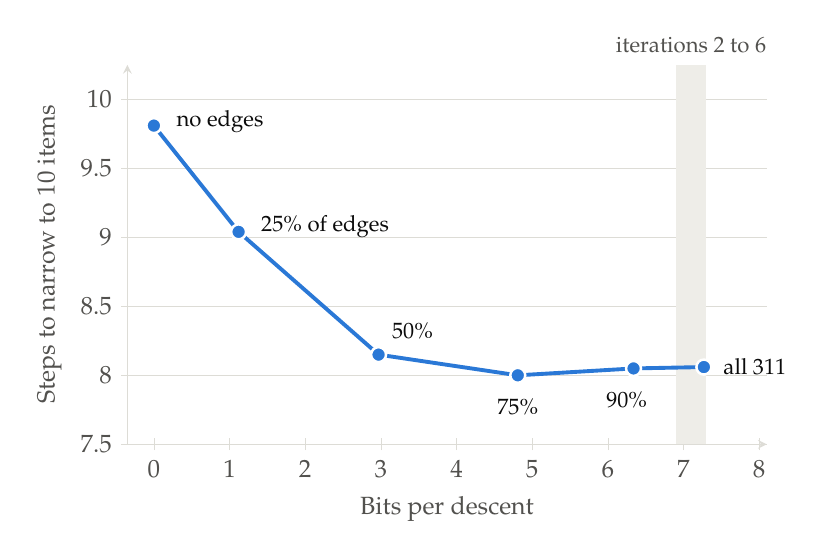
\begin{tikzpicture}
\begin{axis}[
  width=0.80\linewidth, height=6.4cm,
  xmin=-0.35, xmax=8.1, ymin=7.5, ymax=10.25,
  xtick={0,1,...,8}, ytick={7.5,8,8.5,9,9.5,10},
  xlabel={Bits per descent}, ylabel={Steps to narrow to 10 items},
  axis lines=left, axis line style={draw=gridc},
  ymajorgrids, grid style={gridc, line width=0.3pt},
  tick style={draw=gridc},
  tick label style={font=\small, text=muted},
  label style={font=\small, text=muted},
  clip=false,
]
\fill[band] (axis cs:6.9,7.5) rectangle (axis cs:7.3,10.25);
\node[font=\footnotesize, text=muted, anchor=south] at (axis cs:7.1,10.27) {iterations 2 to 6};
\addplot[accent, line width=1.4pt, mark=*, mark size=2.7pt,
  mark options={fill=accent, draw=white, line width=0.9pt}]
  coordinates {(0,9.81) (1.12,9.04) (2.97,8.15) (4.81,8.00) (6.34,8.05) (7.27,8.06)};
\node[anchor=west, font=\footnotesize, text=ink] at (axis cs:0.17,9.84) {no edges};
\node[anchor=west, font=\footnotesize, text=ink] at (axis cs:1.29,9.08) {25\% of edges};
\node[anchor=south west, font=\footnotesize, text=ink] at (axis cs:3.02,8.19) {50\%};
\node[anchor=north, font=\footnotesize, text=ink] at (axis cs:4.81,7.90) {75\%};
\node[anchor=north, font=\footnotesize, text=ink] at (axis cs:6.25,7.95) {90\%};
\node[anchor=west, font=\footnotesize, text=ink] at (axis cs:7.4,8.06) {all 311};
\end{axis}
\end{tikzpicture}
\caption{Navigation stops improving above about 3 bits per descent. Iteration 5 tags under catalogue v4 with
random subsets of its edges; points from 25\% to 90\% are medians over 120 subsets. Steps use the exact facet
ordering of idea 7, and a failed walk counts as 15.}
\label{fig:nav}
\end{figure}

\subsection{Navigation}

The benchmark narrows the whole collection to at most 10 items by choosing facets, with a cap of 15 steps.
On iteration 5 under v4 it succeeds for 82.9\% of 7,902 items.
\begin{itemize}
\item \textbf{Values carry most of it.} Value facets alone reach 75.0\%; child facets alone reach 29.1\%. The edge set adds 5.6 to 7.8 points of reach, and 1.7 to 1.8 steps under the exact ordering of idea 7 (1.0 to 1.2 under the engine's).
\item \textbf{Growth bought little.} From iteration 2 to 5, bits per descent rose from 6.96 to 7.27 while steps did not fall: 7.75, 7.90, 7.77 and 8.06 under the exact ordering. The 25 nodes added after v1 are worth between nothing (tags moved to the parent) and 0.17 steps and 0.9 point of reach (tags dropped).
\item \textbf{Bits can rise for free.} One edge carries 1.94 of the 7.27 bits, and removing it shortens walks by 0.14 steps. On the seed-only structure, deleting the 14,263 tags of the discovered nodes, instead of moving them to their parents, raises bits by 0.60.
\item \textbf{Task B weight does not rank edges.} The 194 edges below 0.3 alone recover 84 to 94\% of what all edges add to reach. The edge set is about twice as large as navigation needs.
\item \textbf{Shortcut edges buy steps, not reach.} Removing all 176 costs 0.35 to 0.56 steps under the exact facet ordering of idea 7.
\end{itemize}

\subsection{The RQ7 classifier}

RQ7 is the only check whose labels were made without the catalogue: 378 coin descriptions with 28 site
categories. A logistic regression on tag features scores 0.480 micro-F1 with the DAG's ancestors and 0.478
without. Value features alone score 0.475 and term-type features alone 0.421. It responds to nodes and
values, not to edges.

\subsection{What can validate a steering change}

\begin{rtable}{Offline checks available today, by kind of change.}
\begin{tabularx}{\linewidth}{@{}P{4.2cm} L L@{}}
\toprule
Change & Usable offline check & Resolution \\
\midrule
Edge added or removed & Paired navigation on a fixed batch, exact ordering & About 0.1 step or 0.5 point of reach \\
Edge re-weighted & None: navigation does not read edge weights & Not applicable \\
Group of nodes or values & RQ7 classifier on tag features & 127 of 132 single nodes move it by at most 0.004, so groups only \\
Node or value added or removed & None without re-tagging & The moved and dropped assumptions disagree \\
\bottomrule
\end{tabularx}
\end{rtable}

Gold-set retrieval cannot judge structure. The relevance of its node queries is defined through the v6 closure, so removing an edge that changes a closure lowers it by construction; its other queries never touch an edge. Navigation has a blind spot too: it uses the same tags with an oracle user,
so tagging errors are invisible to it.

%======================================================================
\subsection{Tagging noise inside every signal}
\label{sec:noise}

Every signal in this report is read from one tagging run, and the run does not repeat. The figures below
come from the 300 gold items, tagged three times by the production tagger under catalogue v6. The first two
were re-derived for this report; the others come from the reviews.

\begin{itemize}
\item \textbf{The tagger disagrees with itself.} Two runs agree at an F1 of 0.54 to 0.56 on (node, value) tags and 0.64 to 0.67 on nodes. An item receives an identical tag set in 6 to 9\% of cases.
\item \textbf{Noise reads as information.} On the same items, bits per descent is 7.38 to 7.40 for the production tagger, 7.21 to 7.31 for the stronger model and 7.17 for the adjudicated gold labels. The least accurate tagger scores highest.
\item \textbf{Nearly half the tags are weak.} 45 to 46\% of production tags carry a confidence below 0.5. On the gold items such tags are right about 14\% of the time, and the label space counts them like any other tag.
\item \textbf{The residual is partly tagger error.} At internal nodes, the gold labels confirm 29\% of the placements that the tagger's own tags make residual (one review).
\item \textbf{Navigation is an oracle benchmark.} On the gold items it succeeds for 95 to 100\% of targets when the simulated user answers from the index's own tags, and for 31 to 37\% when the answers come from a second run of the same tagger (two reviews agree).
\item \textbf{The offline checks reward noise.} One coin-flip tag on every item raises navigation reach from 82.9\% to 87.3\% and cuts the share of identically tagged items from 9.5\% to about 7\%.
\item \textbf{The edges are not distinguished.} Eight random DAGs with the same number of parents per node score $7.25 \pm 0.85$ bits per descent against 7.27, and navigate as well (one review).
\end{itemize}

The consequence runs through the rest of the report. A signal should count only what a second tagging
reproduces, and a validation outcome should be one that added noise cannot raise.

%======================================================================
\section{Principles for steering}

Six principles follow from the evidence, and each idea below applies at least one.
Figure~\ref{fig:loop} shows where each idea acts in the loop.
\begin{enumerate}
\item \textbf{Steer decisions, not headline numbers.} Each of the three metrics has a cheap way up that helps nothing. Use metrics to rank and gate single decisions.
\item \textbf{Prefer signals that are stable and known early.} Stop mass, reach and stop share are known before any discovery call and repeat across the full batches (rank correlation 0.95 to 0.98 for stop mass, 0.89 to 0.94 for stop share). Candidate-level estimates are coarse and biased.
\item \textbf{Every gain needs a price, and a null.} Any split raises entropy, so a test without a cost per node cannot refuse. A price alone is not enough: a random half of the heaviest residual clears the proposed price 19 times over.
\item \textbf{Measure, do not extrapolate.} New children drew about 1.7 times the items predicted at acceptance.
\item \textbf{Count only what repeats.} A signal read from one tagging run counts tagging noise as benefit. Use what a second run reproduces.
\item \textbf{Judge on the same items, with a check that noise cannot raise.} That means use that holds in two runs, agreement between runs at the changed nodes, navigation with a user who is not the index, or raters. Oracle navigation and the RQ7 classifier stay as do-no-harm checks.
\end{enumerate}

\begin{figure}[!htb]
\centering
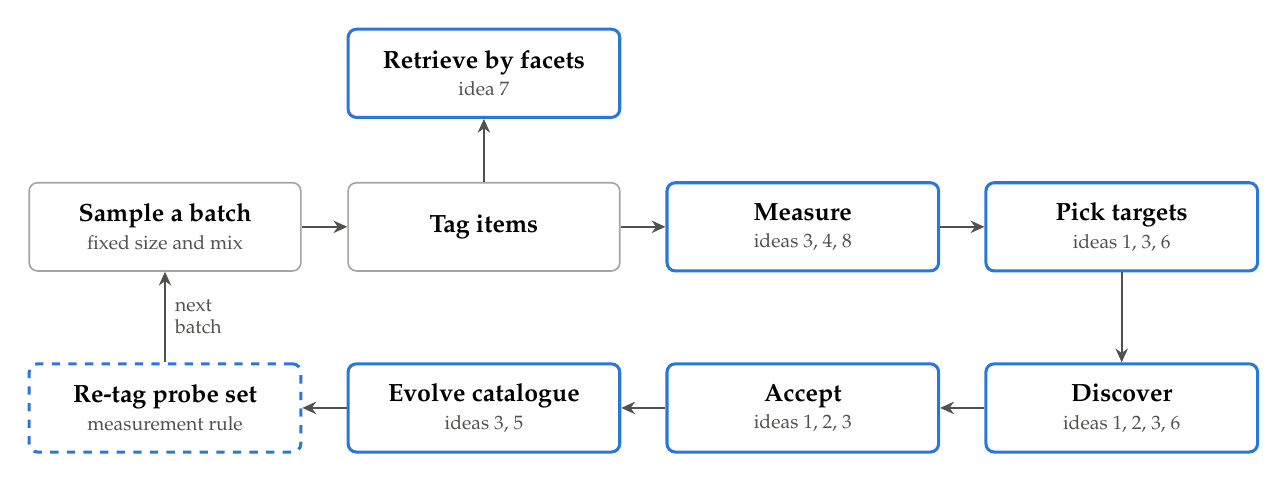
\begin{tikzpicture}[
  font=\small,
  sbox/.style={draw=gridc!60!muted, line width=0.6pt, rounded corners=3pt, minimum width=3.45cm, minimum height=1.12cm, align=center, inner sep=3pt},
  act/.style={sbox, draw=accent, line width=1.1pt},
  new/.style={sbox, draw=accent, line width=1.1pt, dashed},
  arr/.style={-{Stealth[length=5pt,width=4.5pt]}, draw=muted, line width=0.6pt},
  note/.style={font=\scriptsize, text=muted},
]
\node[sbox] (sample) at (0,0) {\textbf{Sample a batch}\\[-1pt]\scriptsize\color{muted}fixed size and mix};
\node[sbox] (tag) at (4.05,0) {\textbf{Tag items}};
\node[act] (measure) at (8.1,0) {\textbf{Measure}\\[-1pt]\scriptsize\color{muted}ideas 3, 4, 8};
\node[act] (targets) at (12.15,0) {\textbf{Pick targets}\\[-1pt]\scriptsize\color{muted}ideas 1, 3, 6};
\node[act] (discover) at (12.15,-2.3) {\textbf{Discover}\\[-1pt]\scriptsize\color{muted}ideas 1, 2, 3, 6};
\node[act] (accept) at (8.1,-2.3) {\textbf{Accept}\\[-1pt]\scriptsize\color{muted}ideas 1, 2, 3};
\node[act] (evolve) at (4.05,-2.3) {\textbf{Evolve catalogue}\\[-1pt]\scriptsize\color{muted}ideas 3, 5};
\node[new] (probe) at (0,-2.3) {\textbf{Re-tag probe set}\\[-1pt]\scriptsize\color{muted}measurement rule};
\node[act] (retrieve) at (4.05,1.95) {\textbf{Retrieve by facets}\\[-1pt]\scriptsize\color{muted}idea 7};
\draw[arr] (sample) -- (tag);
\draw[arr] (tag) -- (measure);
\draw[arr] (measure) -- (targets);
\draw[arr] (targets) -- (discover);
\draw[arr] (discover) -- (accept);
\draw[arr] (accept) -- (evolve);
\draw[arr] (evolve) -- (probe);
\draw[arr] (probe) -- node[note, right, align=left] {next\\batch} (sample);
\draw[arr] (tag) -- (retrieve);
\end{tikzpicture}
\caption{Where each idea acts in the maintenance loop. A blue outline marks a step where an idea changes a
decision. The dashed step does not exist today: re-tagging a fixed probe set under the new catalogue, so that a change is measured on the same items. Probation (idea 4) is decided at the Measure step of the next batch.}
\label{fig:loop}
\end{figure}

%======================================================================
\section{The steering ideas}

\subsection{Idea 1: Screen discovery targets by stop mass}

Use stop mass to decide which nodes discovery visits, in place of the residual-fraction rule. Stop mass is
the share of descents that end at a node; it caps what one new child there can add, in bits, and it is known
before any discovery call. The replay supports it as a screen. It does not support the first version of this
idea, more calls at the heaviest nodes, which the logs cannot test.

\begin{figure}[!htb]
\centering
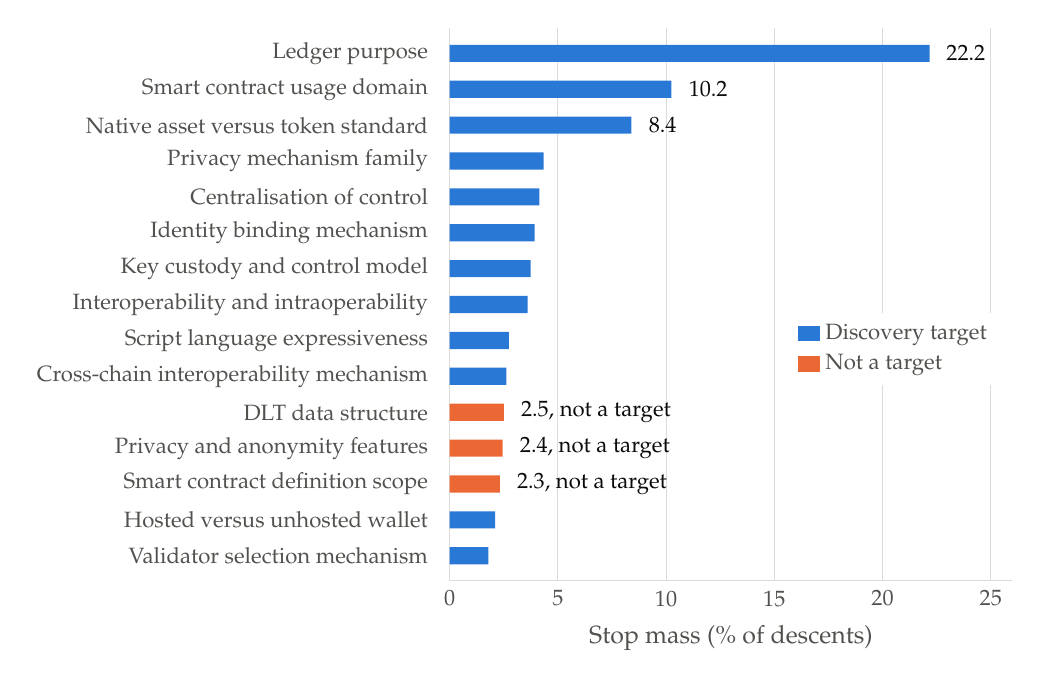
\begin{tikzpicture}
\begin{axis}[
  xbar, bar width=6.2pt, bar shift=0pt,
  width=0.72\linewidth, height=8.6cm,
  y dir=reverse, ymin=0.3, ymax=15.7,
  ytick={1,...,15},
  yticklabels={Ledger purpose, Smart contract usage domain, Native asset versus token standard,
    Privacy mechanism family, Centralisation of control, Identity binding mechanism,
    Key custody and control model, Interoperability and intraoperability, Script language expressiveness,
    Cross-chain interoperability mechanism, DLT data structure, Privacy and anonymity features,
    Smart contract definition scope, Hosted versus unhosted wallet, Validator selection mechanism},
  xmin=0, xmax=26, xtick={0,5,10,15,20,25},
  xlabel={Stop mass (\% of descents)},
  axis x line*=bottom, axis y line*=left,
  axis line style={draw=gridc}, tick style={draw=none},
  xmajorgrids, grid style={gridc, line width=0.3pt},
  tick label style={font=\footnotesize, text=muted},
  label style={font=\small, text=muted},
  legend style={draw=none, font=\footnotesize, text=muted, at={(0.98,0.42)}, anchor=east, legend cell align=left},
  legend image code/.code={\fill[#1] (0cm,-0.1cm) rectangle (0.28cm,0.1cm);},
  clip=false,
]
\addplot[fill=accent, draw=none] coordinates {(22.17,1) (10.25,2) (8.40,3) (4.34,4) (4.15,5) (3.93,6) (3.75,7) (3.61,8) (2.74,9) (2.62,10) (2.10,14) (1.79,15)};
\addlegendentry{Discovery target}
\addplot[fill=accentb, draw=none] coordinates {(2.51,11) (2.45,12) (2.32,13)};
\addlegendentry{Not a target}
\node[anchor=west, font=\footnotesize, text=ink] at (axis cs:22.5,1) {22.2};
\node[anchor=west, font=\footnotesize, text=ink] at (axis cs:10.6,2) {10.2};
\node[anchor=west, font=\footnotesize, text=ink] at (axis cs:8.75,3) {8.4};
\node[anchor=west, font=\footnotesize, text=ink] at (axis cs:2.85,11) {2.5, not a target};
\node[anchor=west, font=\footnotesize, text=ink] at (axis cs:2.8,12) {2.4, not a target};
\node[anchor=west, font=\footnotesize, text=ink] at (axis cs:2.67,13) {2.3, not a target};
\end{axis}
\end{tikzpicture}
\caption{Three nodes hold 41\% of the stop mass, yet each gets the same single call as every other target, and
three of the 15 heaviest nodes were not targets. Iteration 5, catalogue v4; the 15 nodes shown hold 77\% of
the stop mass. Source: \code{output/evolution/iter\_05/maintenance.json}.}
\label{fig:stop}
\end{figure}

\lab{What happens today}
A node is a target when it has at least 5 residual items and a residual fraction of at least 0.3
(\code{maintain.py:298}). Every target gets one call showing up to 40 of its residual items, the most
confident first.
\begin{itemize}
\item \textbf{Leaves qualify automatically.} A leaf's residual fraction is 1, so any leaf with 5 items is a target: 122 of the 202 targets were leaves.
\item \textbf{Light nodes absorb the calls.} 117 of the 202 calls went to nodes whose stop mass is below the price of one node (idea 2).
\item \textbf{Some heavy nodes are skipped.} \code{dlt\_architecture} was a target in iterations 1 and 2. In iterations 3 to 5 it holds 1,062 to 1,153 residual items at a residual fraction of 0.26 to 0.28 and gets no call.
\item \textbf{No sense of size.} In iteration 5, \code{ledger\_purpose} has 5,447 residual items and gets one call showing 40 of them; a node with 5 residual items also gets one call.
\end{itemize}

\lab{The rule the replay supports}
Write $b = \log_2(1 + 1/N)$ for the price of one node in a catalogue of $N$ nodes (idea 2).
\begin{enumerate}
\item Target every node with at least 5 residual items and a stop mass of at least $b/2$. Drop the 0.3 residual-fraction test.
\item Use the same factor in the acceptance price. At the full price, a candidate at a target below it could never be accepted.
\item Drop a candidate that matches an existing value or child of its node, and pool the support of a label that is re-proposed at the same node on later batches.
\item Remember success, not failure. A node that produced a child term type at its last visit produced another on 37\% of visits, against 14\% otherwise. Past failure predicts nothing.
\item As a lighter change, keep today's number of targets and choose them by stop mass.
\end{enumerate}

\lab{Replay on iterations 2 to 6}
\begin{itemize}
\item \textbf{Fewer calls, more mass.} The rule gives 24 to 29 targets per iteration against 32 to 45, covering 91 to 95\% of the stop mass against 82 to 87\%.
\item \textbf{What it keeps.} 97 of the 187 logged calls, 19 of 34 accepted child term types, 37 of 52 accepted values, and 86 to 89\% of the bits those additions delivered on the next batch.
\item \textbf{No miss among the additions that paid.} Ten child term types later cleared the price on the next batch. The rule keeps all ten; leaving one iteration out, nine.
\item \textbf{What it gives up.} 15 accepted child term types and 15 values, among them 12 of the 27 children that meet today's 0.1-bit criterion on the next batch.
\item \textbf{The lighter change.} Choosing today's number of targets by stop mass keeps 138 calls, 32 of 34 child term types and 47 of 52 values.
\item \textbf{Nodes it adds.} Each iteration it brings in 3 to 6 heavy internal nodes that the 0.3 rule skips; they hold 5 to 12\% of the stop mass.
\end{itemize}

\lab{What the replay does not support}
\begin{itemize}
\item \textbf{More calls at heavy nodes.} This is untested, not refuted: no batch has two calls at one node. The 12 calls at the three heaviest nodes returned no child term type.
\item \textbf{Higher yield at heavier nodes.} A call yields a child term type on 17.8\% of calls above the price and 17.5\% below. Heavier nodes do yield more accepted values (30\% of calls against 16\%).
\item \textbf{The screen under today's criterion.} It is supported only if success means clearing a price per node. Under the current 0.1-bit local criterion it gives up 44\% of the children that succeed.
\item \textbf{The added nodes.} Calls at the newly included internal nodes are an experiment. After a child had been accepted at such a node, later calls there yielded 0.17 child term types per call.
\end{itemize}

\lab{Points from the reviews}
\begin{itemize}
\item \textbf{The legal side would starve.} A price skip cuts discovery targets in the actor, activity and obligation categories from 6 to 13 per iteration to 0 to 2, although those categories gave 21 of the 86 acceptances of iterations 2 to 6. A floor per category is needed.
\item \textbf{A budget saves nothing.} A discovery call costs about \$0.001, 1\% of an iteration. Use stop mass to add evidence, not to cut calls.
\item \textbf{Traffic that success cannot lower.} A new child is itself a leaf whose items all stop there, so the heaviest branch stays the top target however often it is split.
\end{itemize}

%----------------------------------------------------------------------
\subsection{Idea 2: Rebuild the acceptance test}

Label a random sample of the residual, check candidates for duplicates, and treat a price per node as a
choice of objective, not a finding. The replay supports the first two. It shows that the proposed score is a
threshold on the node, not a test of the candidate.

\lab{What happens today}
\begin{itemize}
\item \textbf{Three tests.} At least 5 supporting ids among at most 40 shown; a gain of at least 0.1 bits; an evidence span matched in a supporting item.
\item \textbf{The count decides.} It caused 407 of 418 rejections, and 72 of the 94 accepted candidates list exactly 5 ids.
\item \textbf{The share is extrapolated.} For the 311 candidates whose residual exceeds the 40 items shown, the listed ids are scaled up to the whole residual, by a median factor of 4 and up to 141.
\item \textbf{Values get the same test.} A value cannot change the branching gain it is scored by.
\end{itemize}

\lab{What the replay supports}
\begin{enumerate}
\item \textbf{A random, fully labelled sample.} For existing values, the share among the 40 most confident items misses the share in the whole residual by 0.106 on average. A random 40 misses by 0.035 and a random 100 by 0.014.
\item \textbf{A duplicate check.} 15 of the 512 candidates repeat an existing value, an existing child, or a term type elsewhere in the catalogue. Four of them were accepted. The check has one false positive.
\item \textbf{Listing every supporting id.} The prompt asks for ``at least 3'' and acceptance needs 5; 44 of the 48 added values with a next batch list exactly 5.
\end{enumerate}

\lab{What the replay shows about the price}
The score proposed in version 1 was stop mass times the entropy of the split, against a price per node:
\begin{equation}
s\,h_2(f) \;\ge\; \log_2\!\left(1 + \tfrac{1}{N}\right) \approx 0.011 \text{ to } 0.015 \text{ bits for } N = 132 \text{ to } 93 \text{ nodes.}
\end{equation}
\begin{itemize}
\item \textbf{It is a threshold on the node.} With one constant share for every candidate, the decision is the same for 93 of 94. It amounts to a stop mass of 0.021 to 0.028, which 10 or 11 of the 32 to 45 targets clear.
\item \textbf{It is severe.} It keeps 35 of the 94 accepted candidates: 14 term types and 21 values. Applied through the history, 26 of the 39 new nodes would not exist.
\item \textbf{Its error depends on the yardstick.} Against its own target, a realised gain above the price, it is wrong for 5 to 7 of 35 term types. Against today's target of 0.1 bits at the parent, or against next-batch use, it is wrong for 22 to 23 of 35.
\item \textbf{So the logs cannot choose.} Each score predicts its own target on the next batch, because stop mass is stable. Adopting the price is a choice of objective. If it is adopted, it is cheaper to apply it when targets are chosen (idea 1).
\item \textbf{It has no null.} A random half of the residual of \code{ledger\_purpose} scores 0.22 bits, 19 times the price. The rule ``effective leaves per node must not fall'' admits 637 random half-splits before it binds (one review).
\end{itemize}

\lab{What the replay does not support}
\begin{itemize}
\item \textbf{A text-similarity shortcut for the share.} No offline estimator is distinguishable from the logged extrapolation. The intervals are too wide to exclude a real gain, so this is not a refutation.
\item \textbf{A coherence test.} Its pass rate follows the number of listed ids (21\%, 36\% and 51\% at 3, 4 and 5), and it adds nothing to the support count as a predictor of use.
\item \textbf{Pricing values by the DAG score.} Use the stop-mass floor of idea 3 and probation.
\end{itemize}

\lab{Evidence that stands from version 1}
\begin{itemize}
\item \textbf{The estimate is biased low.} New children drew about 1.7 times the predicted items on the next batch.
\item \textbf{The count carries the signal.} The raw support count predicts next-batch use (rank correlation 0.62, interval 0.31 to 0.80). The gain in bits does not ($-0.08$). Both rest on 25 nodes.
\item \textbf{Current additions are mostly real.} 23 of 25 child types accepted in iterations 2 to 4 delivered at least 0.1 bits at their parent on the next batch.
\end{itemize}

\lab{Cost}
Labelling 100 random residual items at each of the 45 targets of iteration 5 means 2,638 items at about
\$0.00054 each, roughly \$1.40.

%----------------------------------------------------------------------
\subsection{Idea 3: Bring values into the metric}

Measure where descents stop at the level of (node, value) cells, and accept a new value when its node
carries enough stop mass. The replay supports the measurement and that simple floor. It does not support a
trigger on dominance, or text clustering as a check before asking. This is the direction in the author's
notes: information gain applied to values, and a value promoted to a term type.

\lab{The measurement}
Let a descent that stops at a node take one more step, into the value its residual item carries there. The
stop distribution is then over (node, value) cells.
\begin{itemize}
\item \textbf{One identity.} Bits per descent and the logarithm of effective leaves both rise by the same amount: the value entropy of each residual, weighted by stop mass. Route multiplicity is untouched.
\item \textbf{Iteration 5.} Bits per descent go from 7.27 to 9.19, and 24.8 effective leaves become 93.7 effective cells.
\item \textbf{Over the iterations.} Effective cells are 33.3, 63.9, 77.4, 88.7, 93.7 and 93.1 in iterations 1 to 6.
\item \textbf{Where the mass is.} 379 of the 491 catalogue cells receive stop mass and the top 25 hold 58\%. Cells the loop created hold 67.6\%.
\item \textbf{Stability.} Cell masses persist between consecutive full batches (rank correlation 0.92 to 0.93).
\end{itemize}
The 8.95 bits and 98.7 leaves quoted in version 1 answer a different question: what if every value became a
child node.

\lab{Accepting a value}
\begin{enumerate}
\item Accept a value when its label is not already a value of the node, its evidence span is found, and the node's stop mass is at least about 0.01.
\item Put accepted values on probation (idea 4).
\end{enumerate}
\begin{itemize}
\item \textbf{The floor on the logs.} It keeps 29 of the 48 values that can be checked on a next batch and is wrong for 10 to 17\% of them (10 to 23\% leaving one out). Accepting everything is wrong for 35 to 46\%.
\item \textbf{The node does the work.} A value-level entropy score tracks the next batch better than the logged score (rank correlation 0.31 to 0.43 against 0.06) but improves no decision.
\item \textbf{Values bring items.} Nodes that received values grew by a median factor of 1.15 on the next batch; comparable nodes shrank to 0.94 to 0.96. An accepted value therefore does move closure-based metrics later, through the tagger.
\item \textbf{Weak values exist.} 6 of 31 added values attracted fewer than 5 items on the next full batch.
\end{itemize}

\lab{Sub-questions under heavy cells}
\begin{itemize}
\item \textbf{Trigger on mass, not dominance.} The 12 collapsed nodes of iteration 5 hold 4.7\% of the stop mass, and only 2 of the 23 heaviest cells are a dominant value of a collapsed node.
\item \textbf{A queue.} 23 cells with a stop mass of at least 0.012 hold 56\% of all stop mass. Each can be sent to discovery for a sub-question, with items sampled at random from the cell.
\item \textbf{What a sub-question must deliver.} A question with $m$ values and entropy $h$ under a cell of stop mass $s_c$ pays when $s_c\,h \ge 0.0116 + 0.0029\,m$ bits. All 23 cells could meet that with an even four-way question.
\end{itemize}

\lab{What the replay does not support}
\begin{itemize}
\item \textbf{Text clustering as a check.} With the true number of clusters, TF-IDF clustering recovers known values at a median agreement of 0.06 on 14 nodes. A null result under a dominant value is therefore uninformative. Sentence embeddings were not tested; the package is not installed.
\item \textbf{Promotion scored on the logged metrics.} Promoting a node's values to child nodes raises bits per descent at 98 of 113 nodes. Measured in cells, promotion at a leaf is exactly neutral.
\item \textbf{The sign of the value score as a test.} The one added value with a negative predicted score realised a positive gain.
\end{itemize}

\lab{Points from the reviews}
\begin{itemize}
\item \textbf{Values are the least reproducible layer.} Two tagging runs agree less on values than on nodes (F1 0.54 to 0.56 against 0.64 to 0.67).
\item \textbf{The code has no promotion.} A value's items cannot move to a new node without re-tagging, and a value cannot be removed without renumbering the codes the tagger answers with.
\item \textbf{Definitions are missing.} 178 values that arrived with new term types have no definition.
\end{itemize}

%----------------------------------------------------------------------
\subsection{Idea 4: Put candidates on probation}

Confirm or retire an addition by the items it attracts on later batches. The replay shows that the rule is
stable and that it changes little: it is a way to undo a choice, not a lever on size, cost or metrics.
Today nothing is ever removed, and no code acts on the candidate status.

\lab{The rule the replay supports}
\begin{enumerate}
\item Count the items an addition attracts, scaled to the standard batch of 8,646 items and its source mix.
\item Confirm at 10 items or more. Retire only when the count is below 10 with an interval that excludes it. Carry undecided cases forward and decide on the pooled count after three batches.
\item Apply the rule to new term types and to separately accepted values. Leave alone the values that arrive as the value list of a new term type.
\item Let a batch of another size or mix confirm provisionally, never retire.
\item Retired means hidden from the tagger's catalogue and kept in the version history. A seed node is never retired.
\end{enumerate}

\lab{Replay on the logs}
\begin{itemize}
\item \textbf{What was added.} Versions 1 to 6 added 39 term types, 54 separately accepted values, and 178 values that arrived with new term types.
\item \textbf{Use on a full next batch.} 1 of 31 new term types drew fewer than 5 items and 3 fewer than 10. For accepted values the counts are 6 and 9 of 33.
\item \textbf{Stable decisions.} At 10 items, all 20 term types with two or more later full batches get the same decision on each. So do 23 of 26 values.
\item \textbf{No warm-up for values.} Later use over first use is 0.99. For term types the logs do not settle it.
\item \textbf{Error on the logs.} 1 of 7 checkable retirements and 1 of 49 checkable confirmations is contradicted later; none of 29 for term types.
\item \textbf{Small effect.} Retiring everything under 10 items (3 nodes and 9 values) moves bits per descent by at most 0.012, navigation by at most 0.008 steps and 0.13 point of reach, and saves 1.7\% of tagging cost.
\item \textbf{A larger saving elsewhere.} Hiding the 13 seed nodes that stay under 10 items in every full batch saves 6.2\% of tagging cost. Nine of them are used on the RQ7 token descriptions, so this is a choice per kind of content.
\end{itemize}

\lab{What the replay does not support}
\begin{itemize}
\item \textbf{A realised-gain bar.} Whether an addition clears it can be read from the node's stop mass at acceptance (area under the curve 0.95), and the verdict on the two heaviest additions flips with the tag assumption.
\item \textbf{Raw counts on a small batch.} On the sixth batch they would retire additions that standardised counts keep.
\item \textbf{Judging bundled values by count.} 76\% of values under nodes of 10 to 49 items fall below 10 by node size alone.
\end{itemize}

\lab{Points from the reviews}
\begin{itemize}
\item \textbf{Use is not correctness.} The most used addition of iteration 4, \code{centralisation\_locus} with 304 items on the next batch, is among the least reproducible nodes measured. Agreement between two runs on a probe should be a second condition.
\item \textbf{No reader honours a status today.} The catalogue block and the validator would have to; history, label space and index can keep the node.
\end{itemize}

%----------------------------------------------------------------------
\subsection{Idea 5: Separate edge plausibility from branching weight}

Keep two numbers per edge: the Task B weight as a plausibility score, and the child's share of the parent's
closure as a branching share. Today one number does both jobs, and new edges get a placeholder of 1.0. This
idea was not replayed; the reviews changed where the second number should live. It answers the note that
new term types need weights as Task B gives them.

\lab{The change}
\begin{enumerate}
\item \textbf{A separate field.} Emit the child's share of the parent's closure, smoothed with 1 to 3 pseudo-counts, in the measurement output. Never write it into the stored edge weight: that field is read by the tagger's prompt, the prior metrics and the retrieval ranking.
\item \textbf{No placeholder.} Give a new edge no Task B weight, print no number for it in the tagger's catalogue, and mark the prior series from version 1 on as mixing estimated weights with a placeholder (\code{evolve.py:74}).
\item \textbf{Plausibility stays semantic.} Keep the Task B weight for whether an edge exists. A Task B style call for discovered nodes costs about \$0.015 per child.
\item \textbf{Review list from co-tagging.} Rank edges by how often child and parent are tagged on the same item, and review the weakest.
\end{enumerate}

\lab{Evidence}
\begin{itemize}
\item \textbf{Task B weights do not work as branching probabilities.} They are worse than a uniform split: divergence 0.181 against 0.130 bits on iteration 5, with the same ordering in all six iterations.
\item \textbf{Content shares are stable.} Shares fitted on one batch cost 0.004 to 0.006 bits on the next. For parents with fewer than 50 placements the error is larger, 0.13 to 0.24 bits.
\item \textbf{The placeholder distorts the prior.} At 1.0, v5 reads 5.02 bits; at the seed median weight of 0.18 it reads 5.27. That shift is as large as the prior's whole movement since v1.
\item \textbf{Placeholders crowd out seed edges.} At the 11 parents with both kinds of child, new edges take 68\% of the prior branching mass against 45 to 47\% realised.
\item \textbf{Co-tagging separates seed edges from unrelated pairs.} The area under the curve is 0.71 for the co-tag share (0.62 after base-rate correction) and 0.81 to 0.84 for lift. The signal repeats: 0.95 between halves of a batch and 0.96 between batches 4 and 5.
\end{itemize}

\lab{Open points}
\begin{itemize}
\item \textbf{Plausibility is assumed, not shown.} Nothing tests the Task B weight as a plausibility score. It correlates 0.21 with co-tagging, and 0.08 after base-rate correction.
\item \textbf{Nothing measurable depends on the weights.} Task B weight does not rank edges by navigation value, and node-query retrieval is slightly higher with every weight set to one (0.568 against 0.546, one review).
\item \textbf{Co-tagging cannot choose parents.} The best-supported node is an existing parent for only 40 to 47\% of children.
\item \textbf{Task B does not transfer as written.} It limits parents to the child's category, and 9 discovered edges cross categories. Its top parent must cite the corpus, which discovered nodes do not have.
\item \textbf{Three seed edges have weight 1.0 with no rationale and no citation.} One is an artefact: for \code{redemption\_risk\_criteria} the model answered ``none'' with probability 1.0, and the zero-total fallback at \code{is\_a.py:104} gave its only listed parent weight 1.0.
\end{itemize}

\lab{Cost}
Content shares are free. A Task B style call for the 39 discovered nodes would cost about \$0.60.

%----------------------------------------------------------------------
\subsection{Idea 6: Identically tagged items, as a monitor}

Groups of items with identical (node, value) tags are a stable symptom, mostly of thin tagging. The replay
shows they cannot be an objective, and supports only a modest use: flagging the few nodes where such items
stop. This was the ``item new topic'' line in the notes.

\lab{Replay on the logs}
\begin{itemize}
\item \textbf{Size.} On iteration 5, 748 of 7,902 items (9.5\%) sit in groups of more than ten with an identical tag set. Across batches 2 to 5 the share is 8.0 to 10.5\%.
\item \textbf{Thin tagging.} 85\% of these items carry one or two tags. An item with one tag is in such a group with probability 73\%; with four or more, never.
\item \textbf{Few nodes.} Nine nodes hold all the stops, and \code{ledger\_purpose} holds 60 to 65\% in every batch.
\item \textbf{Not an objective.} The same number of tags as the catalogue added since v1, placed on random items, gives a share of 7.0\% against 9.5\% for the real labels. One random bit per item gives 7.1\%. Dropping the least confident tags raises it to 14.6\%.
\item \textbf{Unstable for items.} An item in a large group is in one again after re-tagging with probability 0.60.
\item \textbf{Stable for groups and nodes.} 60 of 87 large groups are large again on the next batch, and 14 tag sets that are large in all four batches hold 64 to 67\% of the mass.
\item \textbf{Unseen by discovery.} Of 3,069 such items in iterations 2 to 6, 13 were among the items shown. 68\% sit at \code{ledger\_purpose}, behind a cap of 40 shown out of about 5,000.
\item \textbf{A different list from stop mass.} Seven of the nine nodes rank between 11th and 91st by stop mass. At five of them, holding 23\% of the stops, no candidate could reach the price of idea 2 whatever it captured.
\item \textbf{Little change with growth.} On fixed items, the catalogue steps from v1 to v4 moved the share by between 0.3 and 3.7 points, depending on the tag assumption.
\end{itemize}

\lab{The rule that survives}
\begin{enumerate}
\item On batches of fixed size and mix, flag a node when at least 20 such items have it as their deepest tagged node. This flags 5 or 6 nodes, and every flag recurred on the next batch (15 of 15, counted in sample).
\item Show discovery the group itself, taking groups that were large on two consecutive batches. Neither the confidence order nor a random sample contains it.
\item Keep the support and evidence tests and the duplicate check. Do not score a candidate by the fall of the share.
\item Report the share only at fixed size and mix, together with tags per item.
\end{enumerate}

\lab{Points from the reviews}
\begin{itemize}
\item \textbf{Fix it on the tagger side first.} One review would drop this as a discovery target and send items with at most two tags to a second tagging pass.
\item \textbf{The prize is bounded.} Removing every such group would lift the ceiling on navigation reach by at most 9.5 points.
\end{itemize}

%----------------------------------------------------------------------
\subsection{Idea 7: Order facets by exact expected narrowing}

At retrieval time, rank facets by the narrowing a randomly drawn target would actually experience. The engine
ranks them by a size-weighted formula that misrates facets whose options overlap. This is the one idea that
steers retrieval, not the catalogue. All three reviews keep it.

\lab{What happens today}
The engine scores a facet as the sum, over its options, of the option's share of total option size times the
log of how much it narrows (\code{query.py:213}). When child closures overlap, option sizes sum to more than
the result set. The weights are then not the probabilities of the answers.

The same overlap separates the facet score $N$ from the maintenance branching gain $g$, where $Z_y$ is the sum
of the children's closures plus the residual:
\begin{equation}
N(y) \;=\; g(y) - \log_2\!\frac{Z_y}{|C(y)|}.
\end{equation}
The two are equal only when no closures overlap. The gap reaches 2.92 bits on iteration 5.

\lab{The change}
For each facet, partition the result set by the answer each item would give, and average the narrowing over
items. The answer rule is the benchmark's own: the most specific child that holds the target, else the
residual. In the code, compute both numbers per facet in one pass and sort by the exact one, and move the
answer rule from the benchmark into the engine so that both use one definition.

\lab{Evidence}
\begin{itemize}
\item \textbf{Shorter walks.} The exact ordering saves 0.58 steps on batch 5 (8.64 to 8.06) and 0.70 to 0.74 on batches 2 to 4. Reach is unchanged.
\item \textbf{Larger than any structural edit.} Scored under the exact ordering, the best structural edit tested gains 0.30 steps.
\item \textbf{It changes other conclusions.} Under the engine's ordering, pruning edges below 0.3 appears to save 0.5 steps. Under the exact ordering it costs 0.04 to 0.18.
\item \textbf{On the paper's own index.} Over all 33,581 items of the v6 index it takes the mean from 10.21 to 9.44 questions, with reach unchanged at 74\% (one review).
\end{itemize}

\lab{Open points}
\begin{itemize}
\item \textbf{The gain belongs to an oracle user.} The simulated user answers from the target's own tags. With answers from a second tagging run most walks lose their target (Section~\ref{sec:noise}); the exact ordering still asks fewer questions there, with no loss of reach (one review).
\item \textbf{A step is not a label.} The benchmark counts a facet with 15 options as one step. Labels read per walk should be reported beside steps.
\end{itemize}

\lab{Cost}
None. It is a change to one scoring function, and any navigation-based validation should use it.

%----------------------------------------------------------------------
\subsection{Idea 8: One cost objective}

A single expected-cost objective cannot replace the three metrics. The replay computed it in three forms. No
form has the right sign for every kind of edit, and its verdict on edge edits flips with one modelling
choice. A price per label keeps two limited uses.

\lab{The model}
The form adapts the cost model of
\href{https://www.microsoft.com/en-us/research/publication/automatic-categorization-of-query-results/}{Chakrabarti, Chaudhuri and Hwang (SIGMOD 2004)}
for category trees over query results. Their first term charges the whole item set of a category; here it is
the residual, since a descent that stops at a node has only the residual left to read:
\begin{equation}
\mathrm{Cost}(y) \;=\; P_w(y)\,|R(y)| \;+\; \bigl(1 - P_w(y)\bigr)\Bigl(K\,n_y + \sum_{c} P(c)\,\mathrm{Cost}(c)\Bigr).
\end{equation}

\begin{rtable}{Every term of the cost model is a quantity the loop already computes, except $K$.}
\begin{tabularx}{\linewidth}{@{}L L@{}}
\toprule
Term in the model & Quantity already computed here \\
\midrule
$P_w(y)$, the chance a user stops and reads at $y$ & The stop share at $y$ \\
$|R(y)|$, the items read on stopping (the whole category in the original) & The residual of $y$ \\
$n_y$, the options shown & The number of children of $y$ \\
$P(c)$, the chance of exploring child $c$ & The child's share of the closure \\
$K$, the cost of reading one label against one item & The one free parameter \\
\bottomrule
\end{tabularx}
\end{rtable}

\lab{The three forms replayed}
\begin{itemize}
\item \textbf{Descent form.} The formula as printed, on the random descent.
\item \textbf{Item form, most specific option.} A user looks for one item and always takes the most specific option that holds it.
\item \textbf{Item form, proportional option.} The same user takes an option in proportion to its size.
\end{itemize}

\lab{Replay on the logs}
\begin{itemize}
\item \textbf{The sign depends on the form.} Against navigation steps on random edge subsets, over three batches, the proportional item form has the right sign in 24 of 24 comparisons, the most-specific form the wrong sign in 12 of 12, and the descent form no relation.
\item \textbf{What a price can do that entropy cannot.} At $K \ge 3$ the cost has an interior optimum over edge sets, and an addition can lose with tags held fixed.
\item \textbf{As an acceptance rule it is a size filter.} At $K = 10$ it passes 141 of 512 candidates, 18\% of verdicts flip within the uncertainty of the share, and its verdict matches the next batch at chance level (22 and 15 of 35 nodes under the two tag assumptions).
\item \textbf{A small $K$ accepts nearly everything.} At $K \le 1$ it passes 87 to 99\% of the logged candidates.
\item \textbf{It rewards lost recall.} Keeping only each item's most specific tag gives 0.24 to 0.67 of the cost, with 90\% navigation failure. The cost follows one path per item.
\item \textbf{Removal verdicts are unstable.} The list of nodes to remove changes with $K$. Only one node, with 8 items, is on it at $K = 3$, 10 and 30, and an item count finds that node.
\end{itemize}

\lab{What remains}
\begin{enumerate}
\item Keep the three metrics for reporting, and do not steer by the cost.
\item If a price is reported, use the item form at value level, give labels read and items scanned separately, compare only on the same items, and state $K$ with the batch size.
\item For edges, nominate with the proportional form only, confirm each edit with paired navigation, and keep the shortcut edges.
\end{enumerate}

\lab{Points from the reviews}
A better-founded version would evaluate the cost on the engine's own facet walk, with answers taken from a
second tagging so that a miss has a cost, and add a price per catalogue token. It needs the twice-tagged
probe of Section~\ref{sec:first}.

%======================================================================
\section{Further ideas from the reviews}
\label{sec:further}

The three reviews proposed twelve changes the first list missed (Table~\ref{tab:further}). They are
single-pass proposals and none has been replayed. Most rest on one observation: a second tagging run is the
cheapest source of a null.

\begin{rtable}{Ideas added by the reviews.\label{tab:further}}
\begin{tabularx}{\linewidth}{@{}r P{3.3cm} P{3.6cm} L P{2.4cm}@{}}
\toprule
\# & Idea & What it steers & Signal & Needs \\
\midrule
9 & A reliability map & What the loop does next: reword, merge or retire unreliable nodes before adding new ones & Agreement between two tagging runs, per node and per value & A probe tagged twice \\
10 & Replicate-based acceptance & Acceptance of values and child term types & Information shared by two independent assignment passes over a random residual sample, against a permutation null & Assignment calls \\
11 & Planted placebos & Any acceptance score & The share of known-bad planted candidates that pass & Assignment calls \\
12 & Navigation with an independent user & Validation of every edit & Reach when the index holds one tagging and the answers come from another & A probe tagged twice \\
13 & Verifying the residual & The pools discovery reads & Whether a residual item is confirmed at the node, belongs to an existing child, or does not belong & One short call per sampled item \\
14 & A confidence floor & Every count behind the statistics & The confidence stored on each tag, which the label space ignores & Nothing \\
15 & A candidate ledger & Acceptance and the discovery prompt & The same candidate proposed on separate batches, with pooled support & Nothing \\
16 & A declared descent prior & Which nodes a stop-mass rule targets & Stop mass with roots weighted by content, and with roots weighted equally & Nothing \\
17 & Null rows & What may be claimed & Each statistic on random DAGs with the same in-degrees, and on a coin-flip tag & Nothing \\
18 & A rater audit & The choice of acceptance rule & Blind judgements by two raters on accepted and rejected candidates & Two raters \\
19 & A second pass for thinly tagged items & Tagger coverage & Items with at most two tags & Re-tagging calls \\
20 & A stopping rule & When the loop ends & The share of held-out items that carry an addition of the last version & A probe \\
\bottomrule
\end{tabularx}
\end{rtable}

Four of them have numbers from the logs already.
\begin{itemize}
\item \textbf{The ledger (15).} Of 17 labels that recur at the same node and were never accepted, 8 reach five pooled supporting items with verified evidence.
\item \textbf{The confidence floor (14).} A floor of 0.4 removes 32\% of the tags of batch 5 and takes effective leaves from 24.8 to 20.6, while the stop-mass ranking barely moves (rank correlation 0.96, one review).
\item \textbf{The descent prior (16).} Starting descents in proportion to content gives the three legal-side roots 7.9\% of the mass.
\item \textbf{Verifying the residual (13).} At \code{ledger\_purpose}, 109 items of iteration 5 carry a tagger proposal for a missing value, and none is among the 40 shown to discovery (one review).
\end{itemize}

%======================================================================
\section{Ground rules for measurement}

Nine rules make a steering result interpretable. Only the probe set needs model calls.

\begin{rtable}{Measurement rules for any steering run.}
\begin{tabularx}{\linewidth}{@{}P{6.3cm} L@{}}
\toprule
Rule & Reason \\
\midrule
Compare structures on the same items, tagged twice under each catalogue & With tags held fixed a paired difference is precise (standard error 0.005 bits) but describes tags the tagger would not have produced; two runs of one catalogue agree at an F1 of only 0.54 to 0.56 \\
Hold a fixed probe set and tag it twice under every catalogue version & No single catalogue change has been measured before and after on the same items \\
Keep batch size and source mix fixed & Papers and patents differ by up to 0.52 bits; a 300-item batch reads 0.10 to 0.14 bits low \\
Report expected depth, not AUC & AUC is an exact function of expected depth and of a maximum depth set by one descent in a million \\
Report where descents stop separately from the routes they took & The route term is 56\% of bits per descent; give the figure without shortcut edges once, as a reference row \\
Give both assumptions when a node is removed in a what-if & Moving its tags to the parent and dropping them disagree by 0.1 step and 0.9 point of reach, and neither is a guaranteed bound \\
Use the exact facet ordering in any navigation check, and print the result for an independent user beside it & Under the engine's ordering pruning looks better than it is; with an oracle user, added noise looks like progress \\
Act on per-node levels pooled over batches, not on changes between two & Branching-gain levels persist (0.96 to 0.98); changes in it revert ($-0.52$ to $-0.56$) \\
Print null rows beside every structural number & Random DAGs with the same in-degrees score like the real one, and a coin-flip tag raises reach \\
\bottomrule
\end{tabularx}
\end{rtable}

\lab{The probe set}
The on-topic pool is exhausted: all 36,702 items have been tagged once. The probe set therefore has to be
drawn from items already tagged.
\begin{itemize}
\item \textbf{Draw.} 2,000 items from batches 2 to 4, at 43\% papers and 57\% patents, leaving out the 5,032 items ever shown to a discovery call and the 300 gold items.
\item \textbf{Two runs.} Tag it twice under every version. One run cannot separate the catalogue from the tagger.
\item \textbf{Two halves.} Use one half to choose edits and read the other once per version, so that the probe does not become a training set.
\item \textbf{The legal side.} At the batch mix the probe holds little from the actor, activity and obligation branches; add items from those branches pooled over all batches.
\item \textbf{Size.} About 1,000 items resolve a 0.1-bit difference at two standard errors. For the share of items that carry an addition, 2,000 items tagged twice resolve 2.5 points.
\item \textbf{Cost.} About \$0.56 per 1,000 items per run.
\end{itemize}
A rule on logged levels alone would need a margin of 0.12 to 0.17 bits: two standard deviations of a
difference between two iterations, once the tagger's response to a new version (0.04 to 0.06 bits) is
included.

\lab{Per-node decisions}
A node's branching gain is known to within 0.1 bits (two standard errors) only above about 130 closure items.
For 13 of 89 internal nodes the standard error alone is 0.1 bits or more. Flags such as collapsed or dormant
should hold on several consecutive batches before anything acts on them.

%======================================================================
\section{What not to steer by}

Each quantity in Table~\ref{tab:avoid} has a cheap way to improve that does not improve the taxonomy. None
should be maximised, minimised or thresholded as an objective.

\begin{rtable}{Quantities with a degenerate optimum.\label{tab:avoid}}
\begin{tabularx}{\linewidth}{@{}P{4.3cm} P{4.6cm} L@{}}
\toprule
Do not steer by & Its cheap way to improve & Evidence (iteration 5 unless stated) \\
\midrule
Higher bits per descent & Add arbitrary edges, attach a large node under a root, delete tags, contract hubs & 81\% of possible edge additions raise it; on the seed-only structure, deleting the discovered nodes' tags instead of moving them adds 0.60 bits \\
Higher AUC & Flatten the DAG & A DAG with no edges scores 1.000 \\
Lower AUC & Build chains & Removing shortcuts gives 0.500 with unchanged closures \\
More effective leaves & Flatten the DAG & No edges gives 33.8 against 24.8, while navigation failure rises from 17\% to 25\% \\
More effective leaves per node & Remove nodes & Greedy maximisation removes 105 of 124 nodes \\
Signed leave-one-out bits, to pick removals & Selects hubs and a root & The sign flips for 11 of the 65 internal nodes where the two re-attachment rules differ \\
A threshold on Task B weight & None is optimal & No metric has an interior optimum; weight does not rank edges by navigation value \\
The gain threshold & Nothing changes up to 0.2 bits; above that it selects on the node, not the candidate & In iterations 2 to 6, thresholds from 0 to 0.2 bits accept 89 to 81 candidates (76 at 0.3, 59 at 0.5) \\
Differences between logged iterations & Change the batch & They mix source, size and the tagger's response \\
Metrics from Task B weights & Set new edges to 1.0 & At v5 the placeholder moves prior bits per descent by 0.25, more than its whole movement since v1 \\
Same-tag comparison, to accept additions & Add anything & With tags moved to the parent, no addition scores below zero \\
Gold-set retrieval score, to judge structure & Add edges & Node-query relevance is defined through the closure \\
Fewer identically tagged items & Add any tag, even a random one & One random bit per item cuts the share from 9.5\% to 7.1\% \\
Higher navigation reach with an oracle user & Add tags & One coin-flip tag per item raises reach from 82.9\% to 87.3\% (one review) \\
The score $s\,h_2(f)$ against a price & Split the heaviest residual at random & A random half of the residual of \code{ledger\_purpose} scores 19 times the price \\
Next-batch use alone & Add broad nodes under heavy parents & Use follows the parent's stop mass (rank correlation 0.63, one review), not correctness \\
A cost with a small price per label & Add anything & At $K \le 1$ it passes 87 to 99\% of the logged candidates \\
\bottomrule
\end{tabularx}
\end{rtable}

Two qualifications. Shortcut edges also raise bits per descent, but they save 0.35 to 0.56 navigation steps, so they are not a free gain. And leave-one-out bits near zero, in absolute value, remains a usable marker of removable nodes.

Bits per descent keeps one honest use, as a floor. Below about 3 bits it tracks navigation failure (rank correlation $-0.5$ to $-0.7$). The catalogue has always been far above that.

%======================================================================
\section{What to run first}
\label{sec:first}

Run four steps in order (Table~\ref{tab:steps}). The first is free and the rest cost about \$18 together.
Version 1 proposed going straight to a steered iteration; the replays and reviews show that such a run could
not yet be read.

\lab{Why not a steered iteration first}
\begin{itemize}
\item \textbf{Its outcome favours it by construction.} A rule that selects heavy nodes wins on ``items attracted per added node'', because use follows the parent's stop mass.
\item \textbf{The effect is below the noise.} One iteration's additions are worth about 0.3 point of reach, under one standard error of a 2,000-item probe (0.5 to 1.1 point).
\item \textbf{The proposed outcomes rise with noise.} Oracle reach, the identical-tag share and the entropy figures all improve when random tags are added.
\item \textbf{The score has not passed its own null.} It accepts a random half of a heavy residual.
\end{itemize}

\begin{htable}{The four steps.\label{tab:steps}}
\begin{tabularx}{\linewidth}{@{}c L P{2.6cm} L@{}}
\toprule
Step & What & Cost & What it settles \\
\midrule
0 & Free changes: log stop mass and the value-level figures for every node, add the duplicate check, adopt the exact facet ordering, apply the text corrections of Appendix~\ref{app:sentences}, and add three tables from stored data & \$0 & Removes statements a reviewer could refute, and reports what the logs already support \\
1 & The probe: 2,000 items tagged under v6, 500 of them twice & \$1.41 & The first measurement of v6 on the standard mix; agreement between runs for each node; navigation with an independent user \\
2 & A trial of the acceptance score: the 42 targets and 106 stored candidates of iteration 4, three planted bad candidates per target, and up to 200 random residual items per target assigned twice & about \$1, or \$6 with a second model & Whether any score rejects planted candidates, and whether a measured share removes the 1.7-fold bias \\
3 & Selection at equal size: six catalogues built from v4 and the stored candidates of iteration 5, the same number of additions in each, and 2,000 probe items tagged twice under each & about \$15 & Whether the acceptance rule selects anything, and whether measuring or weighting improves it \\
\bottomrule
\end{tabularx}
\end{htable}

\lab{Step 0: the three tables}
Which of the three tests decided each of the 512 candidates; the use of every addition on the next batch;
and navigation over all targets, with the ceiling set by identically tagged items and the exact ordering.

\lab{Step 2: the planted candidates}
At each target, plant three candidates fixed in advance: a paraphrase of an existing value, a vague
catch-all, and a surface feature such as ``the text is a patent claim''. That gives 126 candidates known to
be bad. The decision rule is also fixed in advance: a score may steer only if it accepts at most 10\% of
them. The realised behaviour of the 18 accepted candidates on batch 5 is already stored, so the same trial
shows whether a share measured on a random sample predicts it.

\lab{Step 3: the arms}
Every arm starts from catalogue v4 and adds 5 child term types and 19 values, the number the logged rule
accepted. Code writes each addition under the node that proposed it, with no consolidation call.

\begin{htable}{Arms of the selection experiment. Each contrast changes one thing.}
\begin{tabularx}{\linewidth}{@{}P{1.6cm} L L@{}}
\toprule
Arm & Additions & Contrast \\
\midrule
C0 & None: v4 unchanged & Baseline \\
A1 & The 24 candidates the logged rule accepted & \\
A2a, A2b & Two random draws from the candidates the rule rejected & A1 against A2: does the rule select anything? \\
A3 & The candidates that capture most of a random residual sample, assigned twice, after the duplicate check & A3 against A1: does measuring help? \\
A4 & As A3, ranked by stop mass times the entropy of the measured split & A4 against A3: does the weighting add anything? \\
\bottomrule
\end{tabularx}
\end{htable}

\lab{Outcomes, fixed in advance}
\begin{itemize}
\item \textbf{Use that repeats.} The share of probe items that carry an addition in both tagging runs.
\item \textbf{Validity.} The share of an arm's 24 additions that two raters, blind to the arm, accept as valid and not a duplicate.
\item \textbf{Secondary.} Agreement between runs at the added nodes; navigation with an independent user; expected depth and effective cells as paired differences against C0; catalogue size and tagging cost.
\end{itemize}

\begin{htable}{Cost of step 3 at list prices.}
\begin{tabularx}{\linewidth}{@{}L r r@{}}
\toprule
Part & Calls & Approximate cost \\
\midrule
Assigning residual samples for arms A3 and A4 & at most 5,280 short calls & \$0.50 \\
Tagging the probe: 6 catalogues, 2 runs, 2,000 items & 24,000 & \$13.00 \\
Tagging the 300 gold items under the 6 catalogues & 1,800 & \$1.00 \\
Optional second model on 200 probe items under three arms & 600 & \$6.40 \\
\bottomrule
\end{tabularx}
\end{htable}

The paper states that the loop's thresholds were constant, so any steered run is a new experiment beside the
logged one. The designs of steps 2 and 3 come from the reviews and have not themselves been checked.

%======================================================================
\section{Implications for the paper text}

Nine statements in the current draft need rewording whether or not any steering is added
(Table~\ref{tab:paper}). Each location was checked against the source.

\begin{rtable}{Statements in the draft that the evidence bears on.\label{tab:paper}}
\begin{tabularx}{\linewidth}{@{}P{2.7cm} P{3.5cm} L P{3.9cm}@{}}
\toprule
Location & The draft says & The evidence shows & Possible fix \\
\midrule
\code{4\_method.tex:} \code{626--629} & Facet narrowing ``is the branching gain'' & Equal only when child closures do not overlap; the gap reaches 2.92 bits on iteration 5 & Say it equals the branching gain for disjoint children, and is lower by $\log_2(Z/|C|)$ otherwise \\
\code{4\_method.tex:521} & The shown items ``are a sample of the residual'' & They are the 40 most confident items, as line 510 says & Sample at random, or drop the extrapolation \\
\code{4\_method.tex:532} & A value candidate ``is scored the same way'' & A value cannot change the gain it is scored by; values are 54 of 94 acceptances & Score values by value entropy, or state the limit \\
\code{4\_method.tex:13} & Candidates are ``discovered at impure nodes'' & Targets are chosen by residual count and fraction, not by value entropy & ``At nodes with a large residual'' \\
\code{3\_problem.tex:40} & A candidate is accepted ``only when it raises that measure'' & Every split raises it; the test decided 3 of 418 rejections & Name the support count as the binding test, or adopt a priced test \\
\code{4\_method.tex:277} & ``AUC separates them'' & AUC is an exact function of expected depth and maximum depth & Report expected depth \\
\code{5\_experiments.tex:} \code{273} & The gain rises ``as discovered nodes absorb residual mass and then settles near seven bits'' & The series mixes batch, size and catalogue; on fixed tags each later step adds 0.01 to 0.18 bits & Report the fixed-batch figures; leave iterations 1 and 6 out of the trend \\
\code{3\_problem.tex:33} & ``Every edge cited'' & 109 of the 279 seed edges and all 41 discovered edges carry no citation; three seed edges have weight 1.0 with no rationale & State the cited share, as RQ2 already does; fix the fallback at \code{is\_a.py:104} \\
\code{4\_method.tex:556}, \code{5\_experiments.tex:} \code{85} & The metrics are ``objectives'' & Nothing optimises them & Call them measures, or report a steering result \\
\bottomrule
\end{tabularx}
\end{rtable}

\lab{Results the logs already support}
\begin{itemize}
\item \textbf{Additions deliver.} 23 of 25 added child types gave at least 0.1 bits at their parent on the next batch. The draft reports no realised gain.
\item \textbf{Unused tables.} \code{tables/objectives\_iter.tex} and \code{tables/navigation.tex} are generated and not included.
\end{itemize}

\lab{A longer list, and names}
The paper review lists 28 sentences with replacement text, most of them about the metrics and the
acceptance test. Appendix~\ref{app:sentences} reproduces them. It also proposes names for the case in which
the metrics are not optimised: ``shape statistics'' for the three, ``branching entropy'' for the gain, and
``stop entropy'' and ``route entropy'' for the two parts of bits per descent.

The same review points to two positives the draft could report from stored data. 32 of the 35 added
dimensions receive at least five items on the next batch. And added dimensions are tagged about as
accurately as seed leaves (F1 against the gold labels 0.61 against 0.55).

\lab{Positioning}
\begin{itemize}
\item \textbf{Closest system.} \href{https://arxiv.org/html/2506.10737v1}{TaxoAdapt} expands on one fixed count threshold of 40 papers and never removes anything. No system found uses an entropy objective to choose between widening and deepening.
\item \textbf{Hand-set thresholds are the norm.} The 5, 0.3 and 0.1 of this loop are in line with published practice, and the paper can say so.
\item \textbf{Naming.} What the draft calls information gain is the quantity \href{https://hunch.net/~coms-4771/quinlan.pdf}{Quinlan (1986)} writes $IV(A)$, later named split information in C4.5: the one gain ratio divides by. A reviewer may raise this.
\end{itemize}

\lab{Structure}
Steering results would sit in RQ3 (Section 5.4) and method Section 4.6. The draft has no limitations section:
\code{6\_discussion.tex} is an ethics paragraph, and RQ3 and RQ4 have no limits paragraph.

%======================================================================
\section{Open questions and limits}

The replays settled which ideas the logs support. Whether any of them improves the catalogue is still open:
no steering rule has been run, and no outcome exists for a candidate that was rejected.

\lab{Settled by the replays}
\begin{itemize}
\item Stop mass works as a screen for discovery targets, but only together with a price at acceptance.
\item That price is a threshold on the node. It does not test the candidate.
\item The 40 most confident items are a biased sample of a residual; a random 40 is three times closer.
\item Values can be measured as cells, and accepted on a stop-mass floor.
\item Probation at 10 items is stable and changes little.
\item A cost objective cannot replace the three metrics.
\item Identically tagged items are not an objective.
\end{itemize}

\lab{Needing the twice-tagged probe}
\begin{itemize}
\item How reliable is each node and value, and do the unreliable ones explain the residual?
\item Does navigation with an independent user rank catalogue versions differently from the oracle?
\item Does a share measured on a random labelled sample predict the next batch better than five listed ids?
\item Does any acceptance score reject planted bad candidates?
\item What do a removed node's tags become under a truly smaller catalogue? The one native check, the pilot tagged under v0, fell outside both assumptions for navigation and between them for bits per descent.
\end{itemize}

\lab{Needing a decision}
\begin{itemize}
\item \textbf{The objective.} Today's local criterion or a price per node. The logs cannot choose, and the two disagree on 22 of 35 additions.
\item \textbf{Category floors.} A stop-mass rule alone would starve the actor, activity and obligation branches.
\item \textbf{Retirement.} The paper states that nothing is removed. Probation changes that for candidates.
\item \textbf{Values in the metric.} Counting cells changes the definitions in Section 4.6.
\item \textbf{Where descents start.} Starting in proportion to closure gives the three legal-side roots 7.9\% of the mass. A uniform start gives them 56\% of the bits, and ranks nodes differently.
\end{itemize}

\lab{Limits of this analysis}
\begin{itemize}
\item Every replay holds the tags fixed, while the tagger would respond to a changed catalogue.
\item The three reviews are single-pass. Their numbers are marked where they are used, and their experiment designs are untested.
\item It covers one domain, one corpus and one tagger model.
\item The gold labels are model-adjudicated with v6 in view; there are no human labels.
\item The legal branches carry little content. In iteration 5, 406, 454 and 112 of 8,646 items have an actor, activity or obligation tag.
\end{itemize}

%======================================================================
\appendix
\section{Glossary}

\begin{rtable}{Terms as used in this report.}
\begin{tabularx}{\linewidth}{@{}P{3.4cm} L@{}}
\toprule
Term & Meaning \\
\midrule
Closure of a node & The items tagged at the node or at any of its descendants \\
Residual of a node & The items in its closure that are in no child's closure; they go no deeper \\
Residual fraction & Residual size divided by closure size \\
Descent & A random walk from a root that, at each node, stops or moves to a child in proportion to closure sizes \\
Reach & The probability that a descent visits the node \\
Stop share & The probability that a descent which reaches the node stops there \\
Stop mass & Reach times stop share: the share of all descents that end at the node \\
Branching gain & The entropy of the options at a node: its children's closure shares and its residual share \\
Bits per descent & The expected sum of branching gains along a descent \\
Effective leaves & Two to the power of the entropy of where descents stop \\
Value entropy, dominance & The entropy of the value distribution among items tagged directly at a node; the share of its most frequent value \\
Collapsed, dormant & Dominance of at least 0.85 with at least 10 direct items; an empty closure \\
Shortcut edge & An edge whose child already reaches the parent through another path \\
Probe set & A fixed set of items re-tagged under every catalogue version \\
Moved, dropped & Two assumptions about a removed node's tags: read as tags on the parent, or deleted \\
Exact ordering & Ranking facets by the narrowing averaged over items, as in idea 7 \\
Cell, effective cells & A (node, value) pair at which a descent stops; two to the power of the entropy of where descents stop, counted over cells \\
Price of a node & $\log_2(1 + 1/N)$ bits for a catalogue of $N$ nodes: the gain at which effective leaves per node do not fall \\
Oracle user & A simulated user who answers every facet from the target item's own tags \\
\bottomrule
\end{tabularx}
\end{rtable}

\section{Related methods}

Each source below was opened and its positive claims checked against the text. That TaxoAdapt never removes a node is read from the absence of any removal step.

\begin{rtable}{Methods the ideas draw on.}
\begin{tabularx}{\linewidth}{@{}P{3.9cm} L L@{}}
\toprule
Source & What it does & Bearing here \\
\midrule
\href{https://hunch.net/~coms-4771/quinlan.pdf}{Quinlan (1986)}, Induction of Decision Trees & Divides information gain by the entropy of the split sizes, to penalise many-way splits & The branching gain is that entropy: a cost term there, the benefit here \\
\href{https://cdn.aaai.org/KDD/1995/KDD95-025.pdf}{Mehta, Rissanen and Agrawal (1995)}, MDL pruning & Prunes a subtree when describing it costs more than it saves & A removal rule with a price per node (ideas 2, 4 and 8) \\
\href{https://staff.icar.cnr.it/manco/Teaching/2006/datamining/articoli/CobWeb.pdf}{Fisher (1987)}, COBWEB & Grows a hierarchy incrementally with merge and split, scored by category utility divided by the number of classes & The operators the loop lacks, with a built-in penalty on width \\
\href{https://www.microsoft.com/en-us/research/publication/automatic-categorization-of-query-results/}{Chakrabarti, Chaudhuri and Hwang (2004)} & Chooses a category tree by expected exploration cost & The objective of idea 8 \\
\href{https://ar5iv.labs.arxiv.org/html/2305.13749}{Wang, Shang and Zhong (2023)}, GoalEx & A model proposes clusters, an assigner marks which samples each supports, an integer programme selects & The propose, assign, select pattern behind idea 2 \\
\href{https://arxiv.org/html/2506.10737v1}{Kargupta et al.\ (2025)}, TaxoAdapt & Expands a taxonomy in depth or width when a count passes 40 papers; never removes & The closest published system: count thresholds, no acceptance statistic \\
\href{https://ar5iv.labs.arxiv.org/html/1603.00772}{Naik and Rangwala (2016)} & Rewires an expert hierarchy in one pass by class similarity and tests it on held-out data; reviews wrapper methods that keep a promote, demote or merge only if classification improves & The validation pattern of those wrapper methods: judge a change on held-out items \\
\href{https://ar5iv.labs.arxiv.org/html/1003.3967}{Golovin and Krause (2011)}, adaptive submodularity & Greedy information-gain questioning is near-optimal when answers are noise-free & The licence for greedy local steps, and its limit: tags are noisy \\
\href{https://ar5iv.labs.arxiv.org/html/1803.04585}{Manheim and Garrabrant (2018)} & Classifies how a metric fails once it is optimised & Most rows of Table~\ref{tab:avoid} are failures of this kind \\
\bottomrule
\end{tabularx}
\end{rtable}

\section{Reproducing the numbers}

The analysis scripts and their outputs are in the session scratch directory:

{\footnotesize\path{/private/tmp/claude-502/-Users-Ryan-ucl-thesis-taxonomy/c200331f-6c4e-48a2-8947-c18ef4d28f6e/scratchpad}}

That directory is temporary; copy it into the repository to keep it. Each of the five analyses and each of
the six replays has one folder for the original pass and one for the independent check. The checks'
corrected findings are the source of the figures from those eleven pieces of work. Costs, corpus counts,
paper line references and the literature rows come from single-pass readings, which a separate fact-check
then re-derived for version 1. Figures taken from the three reviews are single-pass and marked as such.
Costs are list prices applied to the token counts recorded in the logs, not invoices.

\section{Sentences in the draft that a reviewer could refute}
\label{app:sentences}

This list is taken from the paper review, with its proposed replacement text. Locations are files under
\code{paper/sections} unless a path is given. Nine of the locations were also checked independently
(Table~\ref{tab:paper}). The numbers inside the proposed replacements come from the review's own offline
computations; re-derive each before it goes into the paper.

{\small\sloppy
\begin{enumerate}[leftmargin=1.8em,itemsep=0.45em]
\item \textbf{0\_abstract.tex:15-18.} ``grows it only where tagged content raises its information gain ... navigation by the same gain''. The gain test was the sole reason for 3 of 418 rejections; the two quantities differ by up to 2.92 bits. Replace: ``(5) uses the graph as the label space for Web content and grows it where at least five tagged items stop short of every child and share a verified span, and (6) indexes the tagged content on the graph for retrieval and facet navigation''.
\item \textbf{0\_abstract.tex:23.} ``55 values''. The log records 54; 55 is accepted minus added types (paper/scripts/\allowbreak{}task\_a\_tables.py:449). Replace by 54, or say 232 values, 178 of which arrive with the new dimensions.
\item \textbf{0\_abstract.tex:24-25 and 5\_experiments.tex:263-267.} ``dimensions discovered in one iteration are among the most used in the next''. True for the pilot only: its six additions rank 1st to 34th of 99 nodes; those of iterations 2, 3 and 4 rank 26th, 57th and 25th or lower. Abstract: ``the six dimensions added by the pilot are tagged on 64\% of the next batch, later additions on 1 to 8\%''. RQ3: ``(2) What the pilot adds is heavily used: ledger purpose is tagged on 4,890 of the 8,646 items of iteration 2 with a value entropy of 2.2 bits, and 64\% of those items carry one of the six new dimensions. Later additions are narrower: the dimensions added in iterations 2 to 5 are tagged on 5.7\%, 2.3\%, 7.6\% and 1.0\% of the next batch (22\%, 8\%, 12\% and 9\% with added values), 32 of the 35 receive at least five items, and in every iteration the two most used new values account for more than half of the use of all new values.''
\item \textbf{0\_abstract.tex:27 and paper/figures/overview.tex:31.} ``reaches ten items in 10.2 questions''. 10.2 is the mean over all walks, a quarter of which never get there. Replace: ``the highest-narrowing facet reaches ten items for 74\% of targets, in 8.7 questions when it does''. Delete ``(the gain of 4.6)''.
\item \textbf{0\_abstract.tex:28-30, 1\_introduction.tex:101-103, 5\_experiments.tex:303-309.} ``the DAG index lifts retrieval over the same tags without closure''. The lift is on node queries only, whose relevance counts a gold tag at any descendant (taxonomy/evaluation/retrieval\_eval.py:50-56), so a match without closure cannot meet it. On value queries (0.624 against 0.649) and AND queries (0.321 against 0.384) the flat match is ahead. Add that split to the sentence.
\item \textbf{1\_introduction.tex:72-76.} Replace ``accepting only candidates that raise the information gain and are supported by verified evidence'' with ``accepting candidates that at least five residual items support and whose evidence span is found verbatim''.
\item \textbf{1\_introduction.tex:89-91.} Replace with ``a maintenance loop that tags content onto the DAG, measures where items stop and grows the DAG there, and a bitset index that retrieves the tagged content and navigates it by expected narrowing''.
\item \textbf{1\_introduction.tex:97-98 and 5\_experiments.tex:190-194, 208-211.} ``the hierarchy resolves 4.72 bits per descent''. 176 of the 279 edges are implied by longer paths; on the other 103 the same walk has 1.62 bits at an expected depth of 6.6. Replace: ``a random descent under the Task B weights has a path entropy of 4.72 bits, 1.62 once the 176 edges implied by longer paths are set aside''. Caption: ``Bits/desc. is the path entropy of a random root-to-leaf descent''.
\item \textbf{2\_related\_work.tex:31-36.} ``enrichment from a corpus has no criterion for when the taxonomy should change. We require every class and value to cite a verified passage and admit content-derived additions only when they raise a measured information gain.'' TaxoCom, cited there, has a novelty threshold and a rule for the number of new children; TaxoAdapt (ACL 2025, not in references.bib) triggers on the same residual count as this loop; none of the 39 added types or 232 added values carries a citation. Replace: ``Enrichment from a corpus is triggered by novelty or count thresholds and judged by raters [TaxoCom, TaxoAdapt]. We use the same kind of trigger, five residual items with a verified span, cite a verified passage for every seed class and value, and check each addition out of sample, on the batch after the one that proposed it.''
\item \textbf{3\_problem.tex:36-41.} Replace with ``describe where a descent of G through the content stops and, at nodes whose items stop short of every child, propose new values of y or new children of y, accepting a candidate when enough residual items support it and its evidence is verified''.
\item \textbf{4\_method.tex:12-16 and paper/figures/overview.tex:22-23.} ``discovered at impure nodes'', ``navigated by the same gain''. Targets are chosen by residual, not value entropy. Replace: ``discovered at nodes with a large residual''; ``retrieved by set algebra and navigated by expected narrowing''.
\item \textbf{4\_method.tex:179-185.} Replace with ``we attach to it three descriptive statistics of its shape, defined through one random walk: the entropy of the walk, the depth at which it ends and the effective number of nodes it ends at. Nothing in the pipeline optimises them and no step descends the DAG: the tagger sees the whole catalogue at once.''
\item \textbf{4\_method.tex:239-254.} Rename ``information gain'' to ``branching entropy'' and add: ``It is the entropy of the split sizes, which C4.5 calls split information, and not a gain: nothing is measured before and after, and splitting any option raises it.'' Drop ``the total discrimination the DAG holds''.
\item \textbf{4\_method.tex:276-278.} ``AUC separates them''. Replace: ``AUC equals 1 - (E[h] - (1 - F(0))/2)/h\_max, so it carries the expected stopping depth and the maximum depth and nothing else; h\_max is set by the longest chain however little mass reaches it (about one descent in a million on our batches), so we report the expected stopping depth.''
\item \textbf{4\_method.tex:290-293.} Replace with ``On a tree with one root H(r) equals the bits per descent. In general bits per descent + H(root) = H(r) + H(path \textbar{} end); the last term, the entropy of the route given where the walk ends, is 4.07 of the 7.27 bits on iteration 5.''
\item \textbf{4\_method.tex:295-298.} ``Together the three expose three failures of a hierarchy''. Replace: ``We read the three as descriptions, not scores. None has a useful optimum: a transitive shortcut or a deleted tag raises the entropy of the walk, a DAG with no edges has the most effective end nodes, and random DAGs with the same number of parents per node score 7.25 $\pm$ 0.85 bits and 24.6 $\pm$ 5.0 effective end nodes against 7.27 and 24.8 for ours on iteration 5.''
\item \textbf{4\_method.tex:436-440.} Add: ``At a leaf every tagged item is residual, so for the 124 of 202 targets that are leaves the rule reduces to at least five items.''
\item \textbf{4\_method.tex:518-525.} ``because the shown items are a sample of the residual''. They are the 40 most confident, and m is the number of identifiers the model chose to list (the prompt asks for at least three). Replace: ``Support: the model lists the residual items that support the candidate, and at least five of them must be among those shown. Gain: the listed count m is scaled to the residual as if the shown items, which are the most confidently tagged, were a random sample of it; the scaled figure under-predicts what a child attracts on the next batch by a factor of about 1.7.''
\item \textbf{4\_method.tex:531-537.} ``A value candidate is scored the same way''. Replace: ``A value candidate passes the same test, although adding a value changes no closure and so no branching gain; for values the test is a screen on support.'' Add: ``Given the other two thresholds the gain threshold seldom binds: it was the sole reason for 3 of 418 rejections, the support count for 407. The extrapolation was introduced after the first run of iteration 2.''
\item \textbf{4\_method.tex:553-554.} ``a new edge carries weight one until the is-a query re-estimates it''. Never run. Replace: ``a new edge has no Task B weight; we set it to one in the path strength of Section 4.7 and have not re-estimated it (all 41 such edges in version 6), so the prior statistics of versions 1 to 6 mix estimated weights (median 0.18) with this placeholder.''
\item \textbf{4\_method.tex:617-629.} ``which the normalisation absorbs''; ``eq. (facet) is the branching gain ... the objective that grows the DAG also routes a search through it''. Replace: ``For a user who takes the most specific option holding the target, the expected narrowing is the sum over options of (a\_o/n) log2(n/n\_o), with a\_o the number of items whose answer is o. The engine ranks facets by the size-weighted form above, which equals it only when options are disjoint; ordering by the exact form saves 0.8 questions per walk. On the result set C(y) the size-weighted form equals g(y) - log2(Z\_y/\textbar{}C(y)\textbar{}): the branching gain when child closures are disjoint, up to 2.9 bits lower when they overlap.''
\item \textbf{5\_experiments.tex:85-86 (and 4\_method.tex:555-557, 628).} ``objectives''. Replace by ``shape statistics''.
\item \textbf{5\_experiments.tex:270-277.} The bits series mixes batch and catalogue; collapsed nodes are not where discovery goes (collapsed nodes that were targets: 2 of 3, 4 of 11, 1 of 12, 0 of 13, 0 of 12, 1 of 9); dormant counts are 13, 1, 1, 0, 1, 9. Replace: ``Measured from the tags, the walk has 6.96, 7.02, 7.22 and 7.27 bits on the four full batches (standard error 0.02). The 300-item pilot (6.92) and the last batch (7.06; 81\% papers against 43\%) are not comparable with them. With tags held fixed, the nodes added at each step account for 0.08 to 0.18 bits for the three steps to version 4 and 0.01 to 0.02 for the step to version 5. The prior figures (4.72 to 5.02) come from a different walk, with uniform roots and stops only at leaves, and are not a baseline. Collapsed nodes, 3, 11, 12, 13, 12 and 9 per iteration, are led by the DLT data structure with 95 to 97\% of its items on blockchain. They are not where discovery goes: from iteration 3 at most one collapsed node per iteration is a target, and the DLT data structure, the fourth-largest residual pool (about 1,100 items), falls under the 0.3 threshold after iteration 2. The largest pools are leaves the loop added, led by ledger purpose (4,890 to 5,629 items). Dormant nodes number 13, 1, 1, 0, 1 and 9.''
\item \textbf{5\_experiments.tex:289-292.} Add: ``With the extrapolation in place the gain test decides almost nothing: over the six iterations it was the only failed test for 3 of 418 rejected candidates.''
\item \textbf{5\_experiments.tex:376-386.} ``Navigation by facet gain works''; ``The failure is inherited from the edge weights''. Replace: '(2) Taking every one of the 33,581 items as a target, the walk reaches ten items for 74.3\% of targets (77\% of the 300 sampled for the table), in 8.7 questions when it does; ordering facets by the exact expected narrowing reaches the same share in 7.9. (3) The failures are not inherited from the edge weights: 15.2\% of the items share their full set of (term type, value) tags with more than ten others, which caps reach at 84.8\% for any ordering and any edge set and accounts for 59\% of the failed walks, and removing the 194 edges lighter than 0.3 moves reach by half a point. (4) The simulated user answers from the target's own tags. On the 300 gold items the same walk keeps its target for 95 to 100\% of items with that user, 31 to 37\% when the answers come from a second run of the tagger, and 22 to 26\% when they come from the gold labels.'
\item \textbf{5\_experiments.tex:409-410.} Add: ``the figure follows catalogue size (32 types 3.6 bits, 170 types 5.9), not downstream accuracy''.
\item \textbf{7\_conclusion.tex:6-8.} Replace ``by measured information gain'' with ``where items stop short of every child''.
\item \textbf{8\_appendix.tex:19-23.} The gain is predicted, three iteration-1 values predate the extrapolation, and the caption quotes value counts for two iterations only. Replace: ``the number of residual items the model listed in support and the predicted increase in branching gain at that node (iteration 1 computed without the extrapolation); the 54 values added to existing nodes are not listed'', and add the realised columns.
\end{enumerate}
}

\end{document}

